\documentclass[mathserif, 10pt]{beamer}
\usepackage[utf8]{inputenc}
\usepackage{amsmath, amsfonts}
\usepackage{appendixnumberbeamer}



\title[Using ML techniques in phenomenological studies in flavour physics]{Using Machine Learning techniques in\\ phenomenological studies in flavour physics}
\subtitle{Jorge Alda,\\ Universidad de Zaragoza/CAPA \hspace{4em} \texttt{jalda@unizar.es} }
\author[Jorge Alda]{Based on \textbf{JA}, J. Guasch, S. Peñaranda \\
arXiv:2109.07405 [hep-ph]}

\date[CERN Workshop]{5th Inter-experiment Machine Learning Workshop\\ 9-13th May 2022}



\usetheme{Zaragoza}
\usecolortheme{Unizar}
\titlepagelogoA{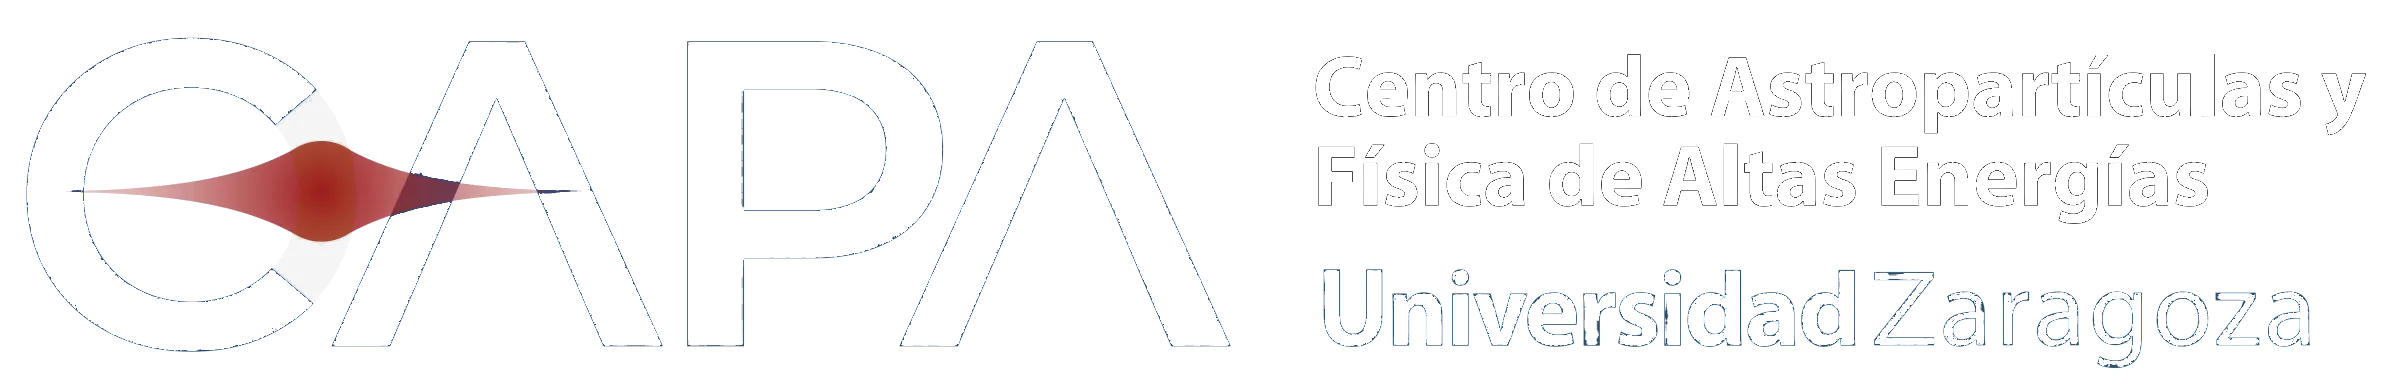
\includegraphics[width=6cm]{logos/CAPA.png}}
\titlepagelogoB{
\includegraphics[width=4cm]{logos/dftuz2.png}}


\newcommand\colorcite[1]{{\scriptsize\color{blue}#1}}

\begin{document}
\begin{frame}[noframenumbering,plain]

\titlepage

\end{frame}

\begin{frame}\frametitle{Problem}
\begin{itemize}
    \item We study $R_{K^{(*)}}$ and $R_{D^{(*)}}$ anomalies
    \item using Effective Field Theory at $\Lambda = 1\,\mathrm{TeV}$.
          $$\mathcal{L}_\mathrm{EFT} = \mathcal{L}_\mathrm{SM} + \frac{1}{\Lambda^2} C \lambda^\ell_{ij} \lambda^q_{kl}\left[ (\bar{\ell}_i \gamma_\mu \ell_j)(\bar{q}_k \gamma^\mu  q_l) + (\bar{\ell}_i \gamma_\mu \tau^I \ell_j)(\bar{q}_k \gamma^\mu \tau^I q_l) \right].$$
    \item Global fits with 5 parameters ($C$, $\alpha^\ell$, $\beta^\ell$, $\alpha^q$, $\beta^q$), log-likelihood function contains 471 physical observables.
\end{itemize}
\begin{columns}[onlytextwidth]
    \begin{column}{0.7\textwidth}
        \begin{itemize}
            \item Non-linear relations $\Longrightarrow$ equi-probability regions are not elliptical $\Longrightarrow$ we can not use Hessian approximation for the log-likelihood.
        \end{itemize}
    \end{column}
    \begin{column}{0.25\textwidth}
        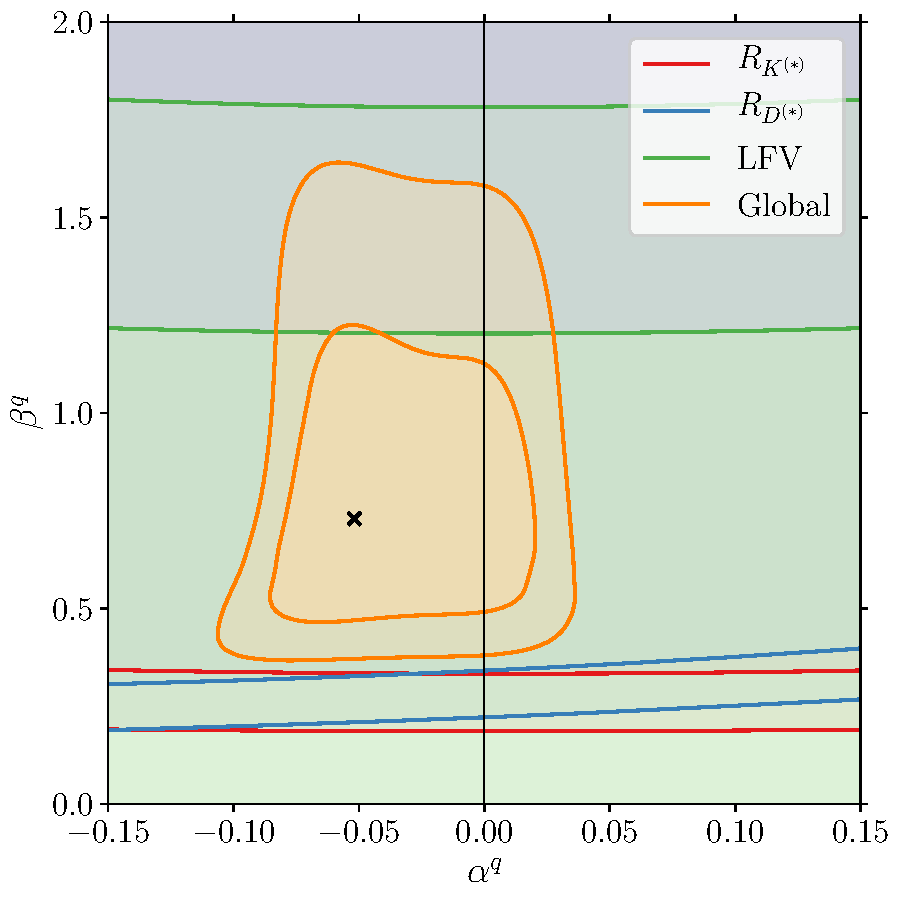
\includegraphics[width=\textwidth]{figures/alphabeta_q.pdf}
    \end{column}
\end{columns}
\end{frame}

\end{document}